\documentclass{amsart}           % use "amsart" instead of "article" for AMSLaTeX format
\usepackage{geometry}                                % See geometry.pdf to learn the layout options. There are lots.
\geometry{a4paper}                                   % ... or a4paper or a5paper or ...
%\geometry{landscape}                                % Activate for rotated page geometry
\usepackage[parfill]{parskip}                    % Activate to begin paragraphs with an empty line rather than an indent
\usepackage{graphicx}                                % Use pdf, png, jpg, or eps§ with pdflatex; use eps in DVI mode
                                % TeX will automatically convert eps --> pdf in pdflatex
\usepackage{amssymb}

%SetFonts
\usepackage{amsmath}
\usepackage{hyperref}
%SetFonts
\newcommand{\me}{\author{Abhay Shankar K : cs21btech11001}
\maketitle}

\begin{document}
    \title{Programming Assignment 2}
    \me
 
    Program flow:
    \begin{itemize}
        \item The main thread reads the values of n and k from the specfied input file, in the function \texttt{io()}.
        \item The \texttt{main()} function then calls \texttt{montecarlo()}, which calculates the number of random numbers that each thread must generate, and calls the \texttt{spawn()} function.
        \item The \texttt{spawn()} function calls \texttt{pthread\_create()} k times, creating k threads which begin in the function \texttt{thread\_init()}.
        \item \texttt{thread\_init()} calls \texttt{gen\_points()}, which generates the required number of random numbers.
        \item The random numbers generated by the string and data about the points (i.e. \# points inside circle, \# points total, etc.) are stored as member fields of \texttt{struct wdata}. Furthermore, they are classified into two \texttt{std::vector}s based on whether or not they are inside the circle.
        \item \texttt{gen\_points()} returns the number of points inside the circle. A semaphore is opened, and this value is added to the global variable \texttt{in\_circle} which combines all the threads' results.
        \item Within the same synchronised block, the \texttt{struct wdata} is pushed onto the global variable \texttt{std::vector rgen}. 
        \item The function \texttt{join\_all()} joins all threads to the main thread, taking a \texttt{std::vector} of pthread\_id as an argument.
        \item Within \texttt{montecarlo()} again, the estimated value of pi and the time taken for the execution of the parallel portion of the code is calculated and printed into the output file.
        \item \texttt{spawn\_io()} is called, and k new threads are formed, beginning in the function \texttt{thread\_io()}. Each io thread writes the random numbers produced by one thread (stored as a single instance of \texttt{struct wdata} within \texttt{rgen}) into a separate file.
        \item The function \texttt{join\_all()} is called again, and all the io threads are joined.
        \item \texttt{montecarlo()} returns, and within \texttt{main()}, \texttt{combine\_files()} is called, and this appends the multiple logfiles produced by the io threads into the output file. It also deletes the intermediate files.
    \end{itemize}

    Benchmarking: 
    \begin{itemize}
        \item Two functions are used: \texttt{clock()} and \texttt{clock\_gettime()}. 
        \item \texttt{clock()} gives the CPU time utilised by the process since it began in $\mu$s - measuring before and after \texttt{spawn()}  and dividing the difference by k yields an upper bound on the CPU time utilised by each computation thread.
        \item \texttt{clock\_gettime()} gives the time elapsed since the Epoch. Measuring twice and subtracting yields an upper bound on the actual time interval during which the MonteCarlo estimation occurs.
        \item Both these times are plotted in the graphs.
    \end{itemize}

    Graphs:
    \begin{itemize}
        \item k variation: \begin{itemize}
            \item CPU 
            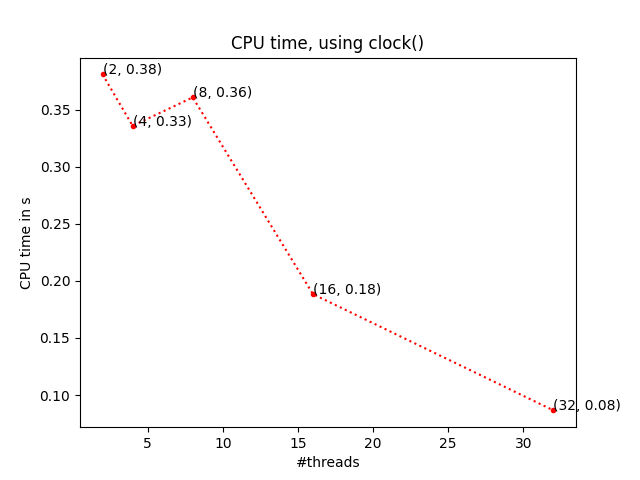
\includegraphics[scale = 0.6]{t_cpu.png}
            \item Realtime
            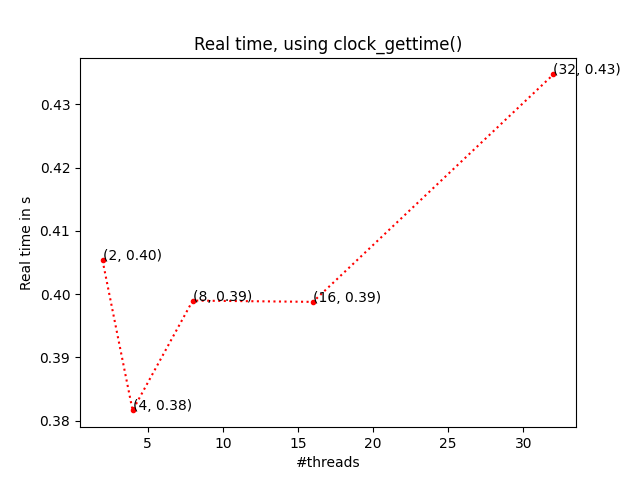
\includegraphics[scale = 0.6]{t_real.png}
        \end{itemize} \newpage
        \item n variation: \begin{itemize}
            \item CPU 
            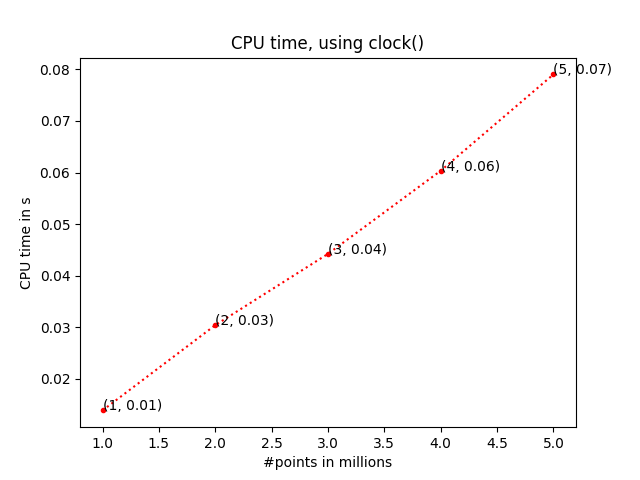
\includegraphics[scale = 0.6]{p_cpu.png}
            \item Realtime 
            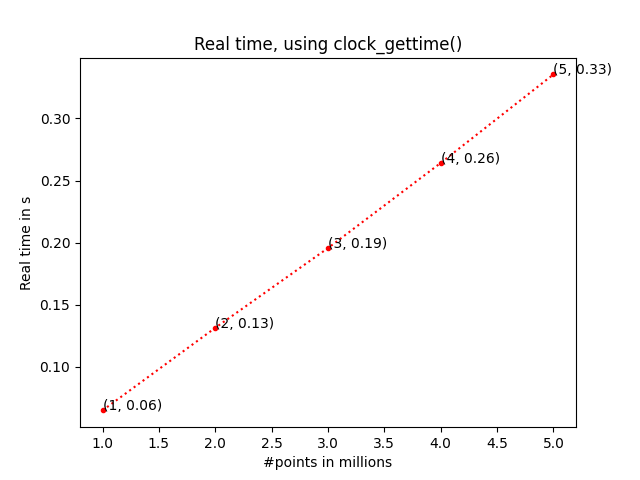
\includegraphics[scale = 0.6]{p_real.png}
        \end{itemize} \newpage
        
    \end{itemize}

    Formats:
    \begin{itemize}
       \item Input: NA
       \item Input file: \texttt{./inp.txt}
       \item Input Format: \texttt{n k}
       \item Output: Value of pi, time taken to compute the value
       \item Output file: \texttt{./output.txt}
       \item Output Format: \texttt{\\
        Value: <pi> \\
        Ticks: <CPU time in $\mu$s>
        Time: <Realtime in $\mu$s>\\
        Thread <num>: <\#Inside circle> <\#Outside circle>\\
        Points inside square: [points] \\
        Points inside circle: [points] \\
        $\vdots$
    }
    \end{itemize}

    Output Analysis:
    \begin{itemize}
        \item The output is an estimated value of pi. 
        \item This estimation is predicated on the fact that computer RNG yields a uniform distribution.
        \item We generate two independent random variables, and due to the ature of uniform distributions, upon plotting these random numbers on orthogonal axes, they are uniformly distributed over a unit square,
        \item Scaling and translating, we get a uniform distribution of points over a square of side length 2 centered at the origin. Because the distribution is uniform, the ratio of areas of this square and the unit circle ($\frac{\pi}{4}$) is equal to the fraction of points within unit distance from origin.
        \item Performing the appropriate arithmetic, we can estimate pi.
    \end{itemize}

    Structs: 
    \begin{itemize}
        \item point: Just a pair of doubles. 
        \item wdata: Contains the entire result of a single thread, including random points classified by their Euclidean norms $\gtrless$ 1, their lengths, and the thread number.
    \end{itemize}
    Functions:
    \begin{itemize}
        \item \texttt{main()}: Minimal functionality. Calls other functions which estimate and print the value of pi. Also prints the time taken by the serial part of the function
        \item \texttt{io()}: Reads the values of n and k from the designated input file and returns them as a \texttt{std::pair}.
        \item \texttt{montecarlo()}: Calls the functions to spawn and join all threads. It also performs the necessary arithmetic, given the number of points within unit distance of origin, to compute pi. Prints the benchmark times as well as the estimate for pi into the output file.
        \item \texttt{spawn()}: Spawns the required number of threads (taken as argument). Stores the pthread\_t id's of the threads in a \texttt{std::vector} (taken as argument). Returns the value of \texttt{clock()} called immediately before the threads are spawned.
        \item \texttt{join\_all()}: Joins all the threads whose pthread\_id is stored in a \texttt{std::vector} taken as argument. Returns the value of \texttt{clock()} called immediately after the threads are joined.
        \item \texttt{thread\_init()}: Calls \texttt{gen\_points()}, stored the generated numbers and the extracted metadata in a \texttt{struct wdata}, and pushes it onto the global \texttt{std::vector}.
        \item \texttt{gen\_points()}: RNG occurs here. Their Euclidean norms are evaluated and, depending on the value, they are pushed onto one of two possible \texttt{std::vector}s. 
        \item \texttt{inside()}: Evaluates the Euclidean norm of a pair of reals.
        \item \texttt{spawn\_io()}: Spawns k threads, storing the pthread\_t id's of the threads in a \texttt{std::vector} (taken as argument). 
        \item \texttt{thread\_io()}: Writes the points from the global \texttt{std::vector} into multiple files using multiple threads.
        \item \texttt{combine\_files()}: Concatenates multiple files produced by \texttt{spawn\_io()}. Cleans up the various intermediate files.
    \end{itemize}
        
\end{document}